In this paper, we employ traditional PERT and CPM concepts to develop a framework for assessing engineering project schedules. However, in this study, we address uncertainty by incorporating possible scenarios, using metrics based on financial risk management: Value-at-Risk and Expected Shortfall, allowing a more realistic analysis of scheduling risk. We analyse uncertainty using Monte Carlo simulation and Bayesian Networks, from a digital twin perspective. 

The following sections present the theoretical background underlying these methods and their applications within the proposed framework. 

\subsection{PERT/CPM and Graphs}

This paper explores PERT and CPM to analyse the risk of the engineering project schedule. The early and seminal works of PERT \citep{Malcolm1959, Clark1962, Elmaghraby1967} and CPM \citep{Kelley1961, Fulkerson1961} provide practical motivation and mathematical underpinnings for these techniques, which are widely used in engineering and construction planning. 

In the following sections, we briefly present the theoretical background underlying these methods and their application within our proposed framework.

 
\subsubsection{Events and Activities}
Engineering projects can be decomposed into a structured set of activities, each representing a well-defined component of the overall work. In a probabilistic scheduling environment, the duration of each activity may be characterised by a probability density function that captures inherent uncertainties. Logical constraints between activities, expressed as precedence relationships, define how these elements are connected within the project network \cite{bagshaw2011, moder2020}. 


In the PERT/CPM formulation, there are two main approaches to represent the precedence of activities in a project 
 \citep{jafari2019, singh2018}: 

\begin{itemize}
    \item Activity on Arc (AOA): Activities are represented by arcs and events by nodes. Each arc shows the duration of the activity. Dummy activities may be used to preserve correct precedence relationships.
    
    \item Activity on Node (AON): Activities are represented by nodes and precedence relationships by arrows connecting them. This approach is generally easier to construct and avoids the need for dummy activities.
\end{itemize}

 
\label{subsec:graph_approach}
%\subsubsection{Graph Approach}

%A PERT/CPM network can be represented as a directed, connected, and acyclic graph \( G(V, A) \), where \( V = \{ v_1, v_2, \ldots, v_n \} \) is the set of nodes (events) and \( A = \{ a_1, a_2, \ldots, a_m \} \) is the set of arcs. %(activities).\textcolor{red}{XXX incluir referencias}
%Events are indexed such that an event \( v_i \) precedes an event \( v_j \), with \( i < j \), whenever an activity exists from \( v_i \) to \( v_j \). 

%The initial event \( v_1 \) and the final event \( v_n \) represent the start and completion of the project.
%In the probabilistic formulation, the duration \( t_k \) of each activity \( a_k \in A \) is modeled as a non-negative random variable, capturing the uncertainty inherent in engineering and construction operations.
%Let \(R = \{ r_1, r_2, \ldots, r_{|R|} \},\) be the set of all simple paths connecting events \( v_1 \) and \( v_n \), where \( |R| \) denotes the cardinality of this set.

%The duration \( T_j \) of a path \( r_j \in R \) is defined as:

%\begin{equation}
%T_j = \sum_{a_k \in r_j} t_k .
%\label{eq:path_duration}
%\end{equation}
%%%%%%%%%%% Marcos Henrique%%%%%
\subsubsection{Graph Approach}
\begin{figure}[h]
    \centering
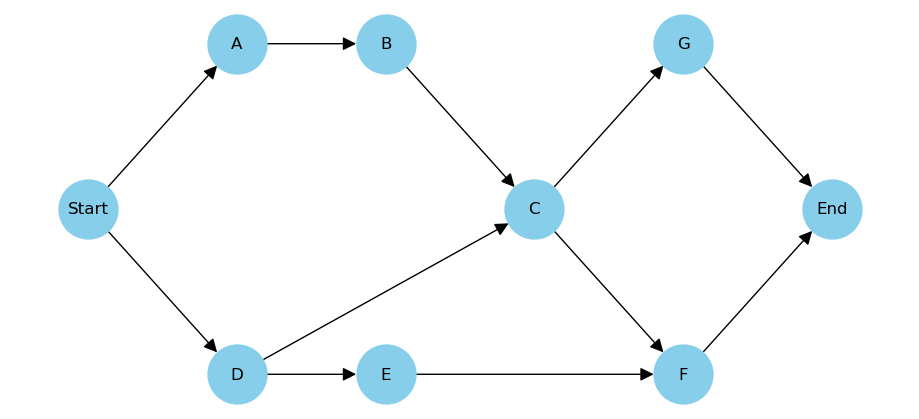
\includegraphics[width=0.6\linewidth]{images/fig_grafo_direcionado.png}
    \caption{Graph of the project plan.}
    \label{fig:031024}
\end{figure}

A PERT/CPM network is represented as a directed, connected, and acyclic graph   
\( G = (V, A) \), where 
\( V = \{ v_1, v_2, \ldots, v_n \} \) denotes the set of nodes, each corresponding to an activity, and 
\( A \subseteq V \times V \) denotes the set of directed arcs representing precedence relations between activities \citep{bagshaw2021pert}. An arc \( (v_i, v_j) \in A \) represents a precedence relation in which activity \( v_j \) starts after the completion of activity \( v_i \), with \( i < j \).

The graph is structured so that \( v_1 \) and \( v_n \) represent the start and completion of the project, respectively, corresponding to dummy activities of zero duration, thereby defining complete execution paths.

In the probabilistic formulation, the duration \( t_i \) associated with each activity node \( v_i \in V \) is modelled as a non-negative random variable, capturing the uncertainty inherent in engineering and construction operations.

Let \( R = \{ r_1, r_2, \ldots, r_{|R|} \} \) denote the set of all simple paths that connect the initial activity \( v_1 \) and the terminal activity \( v_n \), where \( |R| \) denotes the cardinality of this set.

The duration \( T_j \) of a path \( r_j \in R \) is defined as the sum of the durations of the activities along the path:
\begin{equation}
T_j = \sum_{v_i \in r_j} t_i .
\label{eq:path_duration}
\end{equation}

%%%%%%%%%%%%%%%%%%%%%%%
\subsubsection{Critical Path}

The duration of a schedule is determined by the temporal constraints of the network activities. That if there is a path from the origin event ($v_1$) to the terminus event ($v_n$) whose length equals the duration of the schedule, this path is designated as a \textit{critical path} \citep{Kelley1961}.

Mathematically, considering the set of all path durations computed in Eq. (1), the project duration ($T_{project}$) corresponds to the maximum value among all possible paths $r_j \in R$. Thus, the critical path determines the minimum time required to complete the project:

\begin{equation}
T_{project} = \max_{r_j \in R} \{ T_j \} \quad (2)
\end{equation}

Activities located on this path are termed \textit{critical activities}. These activities are limiting in that any delay in one of them will cause a comparable delay in project completion \citep{Kelley1961}. In terms of float analysis, critical activities are characterised by having a total float equal to zero, meaning the maximum time available for the activity equals its duration.

Since this study considers the durations of activities $t_k$ as random variables, the inequality $T_{project} \ge T_j$ holds for all $j$, but the specific path that satisfies the condition of maximum duration can vary between different simulation scenarios.

\label{sub:var}
\subsection{Risk management metrics}
We briefly discuss two very common risk management metrics, Value--at--Risk and Expected Shortfall), that are extensively used in the finance industry. These metrics are used by banks and regulators to quantitatively assess market, credit, and operational risk, and their concepts can be adapted for the construction industry. 


\subsubsection{Value--at--Risk}

Introduced by J.P. Morgan and Reuters in the 1990s, Value-at-Risk (VaR) is a risk metric now widely used in finance and adapted to other industries. The $VaR$ is based on quantiles of the profit-and-loss distribution of a financial portfolio and measures the amount a portfolio or asset might lose over a specified time horizon with a given confidence level \citep{Riskmetrics}.

Although originally applied to assess potential monetary loss, the concept $VaR$ can also be utilised in other non-financial applications. In our study, we use the quantile interpretation of $VaR$ based on confidence level to analyse the risk of scheduling.   

%Com a amostragem probabilistica de dias X que uma dada atividade pode durar é possível determinar com um nível de confiança $\alpha$ que aquela atividade dure até ${{VaR}_{\alpha}}$ dias.
 
Within this a probabilistic approach, if $X$ is a random variable that describes the duration (e.g. number of days) of an activity of the project, and $1-\alpha$ is the confidence level (e.g. $1-\alpha=95\%$, where $\alpha=5\%$ is the tail probability), then the $VaR$ is the $\alpha$--quantile of the loss distribution, at a confidence level $1-\alpha$, and is defined as:
 
\begin{equation}
    P(X > \text{VaR}_{\alpha})= \alpha
\end{equation}

In the scheduling context, $VaR$ measures the tail probability of an activity's duration (i.e., the maximum duration) at a given confidence level. 

\subsubsection{Expected Shortfall}
The Expected Shortfall ($ES$), also called Conditional Value-at-Risk ($CVaR$), is another widely used risk metric in finance that indicates the expected loss conditional on exceeding the $VaR$ \citep{Artzner1999, Acerbi2002}. From a scheduling perspective, $ES$ identifies the expected value of the duration of an activity conditional on exceeding $VaR$. 

\begin{equation}
ES_{\alpha}(X) = \mathbb{E}\!\left[\, X \mid X \ge \text{VaR}_{\alpha}(X) \,\right]
\end{equation}

Therefore, $VaR_{\alpha}$ would express the maximum duration of an activity, with a predefined confidence level $1-\alpha$, while $ES_{\alpha}$ expresses the expected value of the duration of the activity, in the case it lasts longer than $VaR_{\alpha}$.

\subsection{Bayesian Network and Evidence Propagation}

To formally model the dependencies and uncertainties within [the system under study], we employ a \textbf{Probabilistic Graphical Model (PGM)}, specifically a Bayesian Network (BN). PGMs provide a robust formalism for representing complex stochastic systems by combining principles from graph theory and probability theory.

A Bayesian Network is formally defined by two components. The first is a qualitative structure, a Directed Acyclic Graph (DAG) $\mathcal{G} = (\mathbf{V}, \mathbf{E})$, in which nodes $\mathbf{V}$ correspond to random variables and directed edges $\mathbf{E}$ represent conditional dependencies \citep{caetano2024resilience}. 

The structure of this DAG is fundamental because it encodes a set of conditional-independence assumptions over the domain. These assumptions, in turn, enable an efficient decomposition of the joint probability distribution over the set of all variables $\mathbf{X} = \{X_1, \dots, X_n\}$. Instead of relying on the full chain rule of probability, the distribution factorises according to the graph structure:

\begin{equation}
P(X_1, \dots, X_n) = \prod_{i=1}^{n} P(X_i | \text{pa}(X_i))
\end{equation}

where $\text{pa}(X_i)$ is the set of parents for node $X_i$ in $\mathcal{G}$. The second component of a BN is a set of quantitative parameters, consisting of a Conditional Probability Table (CPT) for each node $X_i$. Each CPT quantifies the local distribution $P(X_i | \text{pa}(X_i))$, completing the probabilistic specification of the model. This factorisation is the core strength of BNs, drastically reducing the complexity of representation and inference.

\subsection{Probabilistic Inference and Evidence Propagation}
\label{subsec:evidence_propagation}

A primary application of Bayesian Networks is probabilistic inference, which involves updating the beliefs about certain variables upon observing new information, known as \textbf{evidence}. This process, often termed \textbf{evidence propagation} or belief updating, allows the model to perform diagnostic and predictive reasoning \citep{pearl1988probabilistic}.

Formally, let the set of all variables in the network be $\mathbf{X} = \{X_1, \dots, X_n\}$. Evidence, denoted as $\mathbf{e}$, is an instantiation of a subset of evidence variables $\mathbf{E} \subseteq \mathbf{X}$ to specific states. The objective of inference is to compute the posterior probability distribution of a set of query variables $\mathbf{Q} \subseteq \mathbf{X} \setminus \mathbf{E}$, given the evidence $\mathbf{e}$. That is, our goal is to compute $P(\mathbf{Q} | \mathbf{E} = \mathbf{e})$.

The foundation for this belief update is Bayes' theorem. For a single query variable $X_i$ and a set of evidence $\mathbf{e}$, the posterior probability is calculated as follows \citep{pearl2022external}:
%
\begin{equation}
\label{eq:evidence_prob_update}
\underbrace{P(X_i | \mathbf{e})}_{\text{Posterior}} = \frac{\overbrace{P(\mathbf{e} | X_i)}^{\text{Likelihood}} \cdot \overbrace{P(X_i)}^{\text{Prior}}}{\underbrace{P(\mathbf{e})}_{\text{Evidence}}}
\end{equation}
%
In Equation \ref{eq:evidence_prob_update}, each term has a distinct role:
\begin{itemize}
    \item $P(X_i)$ is the \textbf{prior probability} of $X_i$, representing the belief about the variable before any evidence is observed. It can be computed from the joint distribution defined by the BN.
    \item $P(\mathbf{e} | X_i)$ is the \textbf{likelihood}, which quantifies the probability of observing the evidence $\mathbf{e}$ for each possible state of the query variable $X_i$.
    \item $P(X_i | \mathbf{e})$ is the \textbf{posterior probability}, representing the updated belief about $X_i$ after considering the evidence.
    \item $P(\mathbf{e})$ is the \textbf{marginal likelihood} of the evidence, which acts as a normalisation constant to ensure that the posterior probabilities sum to one.
\end{itemize}

The marginal likelihood $P(\mathbf{e})$ is computed by summing the joint probabilities over all possible states of the query variable $X_i$, an application of the law of total probability. Assuming $X_i$ can take on states $\{x_{i1}, \dots, x_{ik}\}$, it is given by:
%
\begin{equation}
\label{eq:sum_denominador}
P(\mathbf{e}) = \sum_{j=1}^{k} P(\mathbf{e} | X_i = x_{ij}) P(X_i = x_{ij})
\end{equation}
%
This framework allows for the computation of probabilities that are often difficult to assess directly, such as $P(X_i | \mathbf{e})$, by leveraging more intuitive or empirically derivable quantities like the prior and the likelihood \cite{caetano2024resilience}.